%packages a utilizar:
\documentclass{report}
\usepackage[T1]{fontenc}     % Fontes T1
\usepackage[utf8]{inputenc}  % Input UTF8
\usepackage[top=3cm,bottom=3cm,left=3cm,right=2.5cm,asymmetric]{geometry} %fronteiras
%\usepackage[nottoc]{tocbibind}
\usepackage[table]{xcolor} %Colorir tabelas
\usepackage[backend=biber, style=ieee]{biblatex} %bibliografia
\usepackage{csquotes}  % referências
\usepackage[portuguese]{babel} %Usar língua portuguesa
\usepackage{blindtext} 
\usepackage[printonlyused]{acronym}  %Acrónimos
\usepackage{hyperref}  %Autoref no índice
\usepackage{graphicx}  %Usar imagens
\usepackage{titling}
\usepackage{multicol} %multicoluna de texto
\usepackage{adjustbox}
\renewcommand{\figurename}{Fig.} 
\renewcommand{\tablename}{Tabela} 
\usepackage[font=small,tableposition=top]{caption} 
\usepackage[font=small]{subcaption}
\usepackage{xcolor} %cor nos textos
\usepackage{amsmath} %matematica
\usepackage{amssymb} %simbolos matematicos
\graphicspath{ {./images/} } %directorio das imagens
\usepackage{fancyhdr}
\usepackage{authblk}
\usepackage{float} %Posicionamento exacto das figuras no texto
\usepackage{url}   %referencias URL
\usepackage{blindtext}
\def\UrlBreaks{\do\/\do-} %não cortar referencias

\usepackage{indentfirst} %Garantir avanço do primeiro parágrafo
\hypersetup{pdfborder=0 0 0} %Remover a caixa vermelha das referências
\usepackage{chngcntr} %Numeração contínua das figuras
\counterwithout{figure}{chapter} %Numeração contínua de figuras
\counterwithout{table}{chapter} %Numeração contínnua de tabelas
\setlength{\parskip}{0.2cm} %Aumento de espaçamento entre parágrafos

\usepackage{hyperref}

 
\begin{document}	
	%Definições do Relatório

%Dados Gerais:
\def\titulo{Projecto Final: \\ Máquina de Lavagem de Roupa}
\def\data{Junho de 2022}
\def\versao{Ver.: 1.13}
\def\departamento{Departamento de Electrónica Telecomunicações e Informática}
\def\empresa{Universidade de Aveiro}
\def\logotipo{logotipo_ua.png}

%Dados dos Autores:
%primeiro autor:
\def\pautor{João Pedro Nunes Vieira} 
\def\numpautor{Nº Mec.:  50458}
\def\contactopautor{joaopvieira@ua.pt}
%segundo autor:
\def\sautor{Leandro Roque Costa} 
\def\numsautor{Nº Mec.: 110326}
\def\contactosautor{lrc@ua.pt}
%
\def\autores{\pautor \\ \sautor}

		
%########################################################	
%HEADERS & FOOTERS:
\pagestyle{fancy}
\fancyhf{}
\rhead{\uc}
\lhead{\titulo}
\cfoot{\thepage}

 \begin{titlepage} 
	\begin{center}
	\includegraphics[scale=0.50]{\logotipo}
	\line(1,0){350} \\ 
		\vspace*{2mm}
	{\Huge \titulo} \\
		\vspace*{1mm}
	\line(1,0){350} \\ 
		\vspace*{2mm}
	{\Large \uc \data \\ \Large \vspace{2mm} \tipo \grupo} \\
		\vspace*{20mm}
	{\large \autores} \\ 
	\end{center}

%########################################################	
%########################################################	
%RESUMO%
\section*{Resumo}
\line(1,0){460} \\
Esta atividade laboratorial foi dividida em duas partes, cada uma com objetivos individuais.
\par O objetivo da primeira parte é calibrar uma sonda de efeito de Hall recorrendo a um solenoide padrão por forma a descobrir a constante de proporcionalidade que relaciona o campo magnético e a diferença de potencial. 
\par Na segunda temos três objetivos diferentes: 
	\begin{enumerate}
\item Medir o campo magnético ao longo do eixo de duas bobinas. 
\item Estabelecer a configuração de Helmholtz e medir o campo magnético ao longo do eixo das mesmas bobinas 
\item Verificar o princípio da sobreposição.
	\end{enumerate}
	Em suma, pretende-se verificar as características físicas do campo electromagnético ao longo do eixo central das bobinas de Helmholtz e verificar o princípio da sobreposição. Observou-se que o campo magnético era máximo no seu centro das bobinas e diminuía à medida que a distância ao centro aumentava. \\ 
	Na acopulação das bobinas em série, verificou-se o mesmo resultado, demonstrando assim o principio de sobreposição. \\
\line(1,0){460} \\

\end{titlepage}

%########################################################	
%########################################################	
%INTRODUÇÃO

\section*{Introdução:}

Um solenóide é constituído por um fio condutor enrolado em espiral, cujos anéis são idênticos do ponto de vista físico, colocados lado a lado e percorridos pela mesma corrente. Um solenóide é considerado \textbf{padrão} se cumprir as seguintes condições: 
\begin{enumerate}
\item É conhecido o número de espiras por unidade de comprimento;
\item Tendo o solenóide dimensões finitas, o seu comprimento  é muito superior à medida do raio.
\end{enumerate} 
Assim é possível utilizar a fórmula de campo magnético de um solenóide infinito que é dado por: \\ 
$B=\mu*(N/l)*I (T)$ \\

As bobinas de Helmholtz, são um outro dispositivo que, sendo constituído por duas bobinas similares com aneis de corrente, permite criar um campo magnético mais uniforme do que o campo constituido por apenas uma bobina. \\
Esta característica é resultante quando as bobinas são, idênticas (mesmo raio e número de espiras), coaxiais, e estejam situadas entre si a uma distância igual ao seu raio, sendo a expressão usada para o calculo do campo magnético associado a seguinte:
$B(x)=( \mu /2)*(I*R^2)/(R^2 + (R/2)^2 )^(3/2)$ \\

\section*{Procedimento experimental}
\subsection*{Parte A: Calibração da sonda de Hall}
Montou-se o circuito da Figura 2 para executar a calibrar a sonda de Hall:

\begin{figure}[H]
		\centering
		\begin{subfigure}[t]{0.45\textwidth}
			\centering
			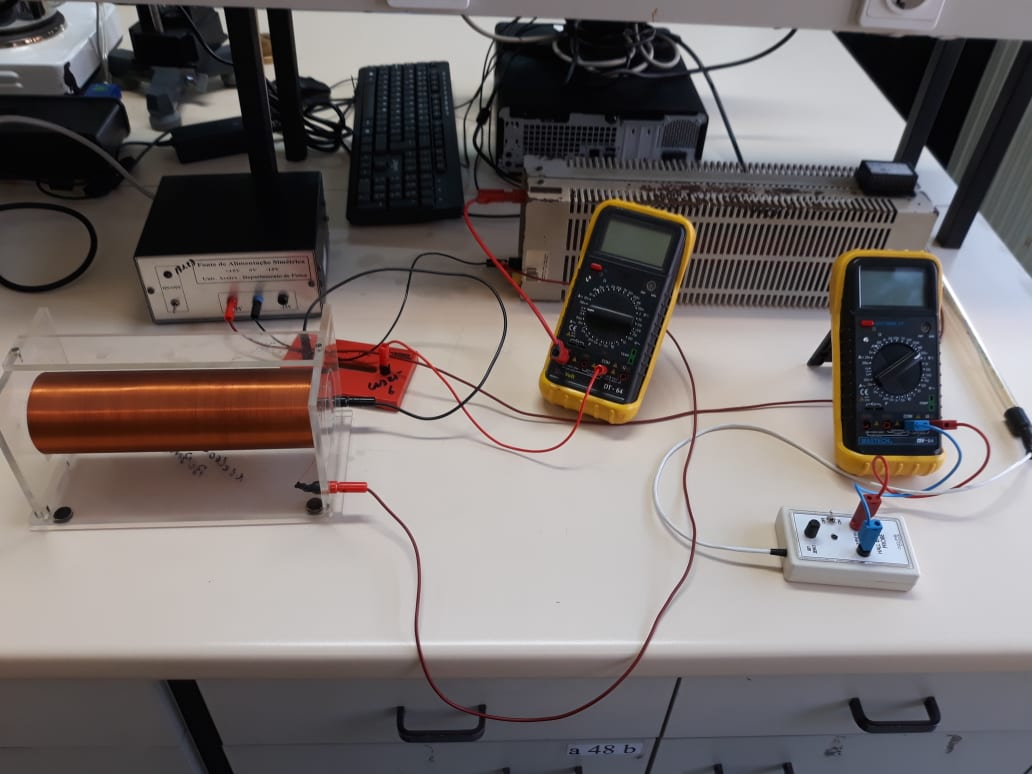
\includegraphics[scale=0.15]{./circuito_A.jpeg}
			\caption{}
		\end{subfigure}
		\begin{subfigure}[t]{0.45\textwidth}
			\centering
			{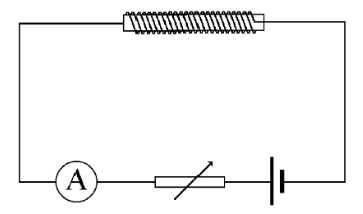
\includegraphics[scale=0.6]{./circuito1.png}}
			\caption{}
			\end{subfigure}	
		\caption{(a) Circuito real montado ; (b) Diagrama do circuito real montado }
	\end{figure}

\small 
Nota: Fechando o circuito, ligamos o terminal da sonda à entrada do amplificador e um voltímetro à saída do amplificador, sendo necessário anular a tensão residual no potenciómetro. \\
\normalsize 
\par Colocando a sonda no interior do solenóide, à medida que aumentamos o valor da corrente elétrica, registámos o valor apresentado no voltímetro (Vh) \textit{documento Excel}, conseguindo assim obter o campo magnético do solenoide e a sua representação gráfica, calculando assim a constante de calibração \textbf{(Cc)}. \\

\subsection*{Parte B: Verificação do princípio de sobreposição para o campo magnético}

\par No início colocamos duas bobinas numa disposição simétrica de acordo com a configuração de Helmholtz, tal como ilustrado na imagem seguinte.


\begin{figure}[H]
		\centering
		\begin{subfigure}[t]{0.45\textwidth}
			\centering
			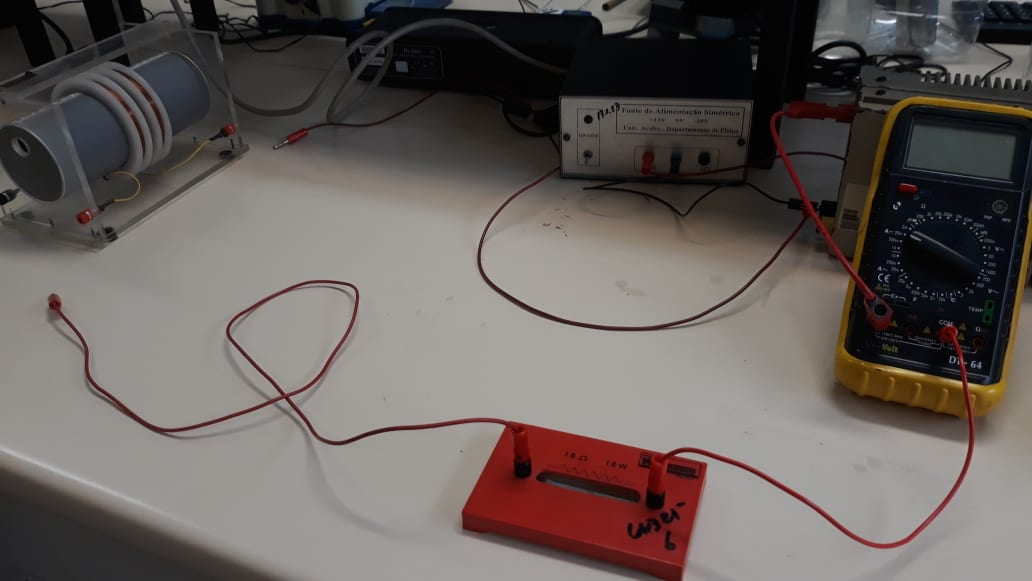
\includegraphics[scale=0.2]{./circuito_B.jpeg}
			\caption{}
		\end{subfigure}
		\begin{subfigure}[t]{0.45\textwidth}
			\centering
			{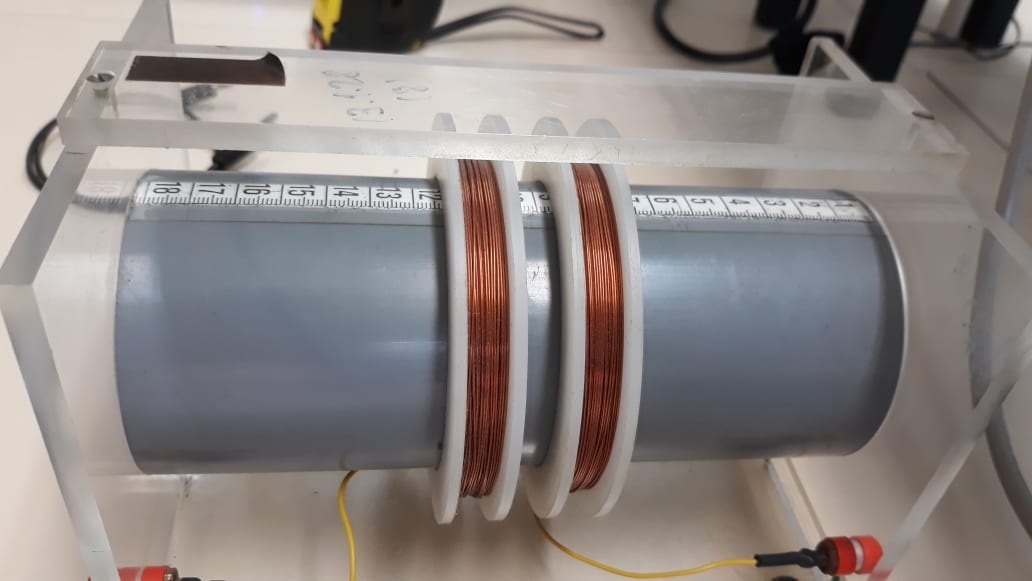
\includegraphics[scale=0.2]{./bobinas.jpeg}}
			\caption{}
			\end{subfigure}	
		\caption{(a) Circuito (aberto) real utilizado ; (b) Bobinas de Helmholtz}
	\end{figure}
	

\small Nota: Esta disposição deve-se manter no resto do procedimento \\

Construímos um circuito em série com uma fonte de 15V, uma das bobinas, o reóstato e um amperímetro parecido ao usado na parte A. A intensidade da corrente deve ser igual a 0,5A. \\
Com a sonda de Hall determinamos o campo eletromagnético criado pela bobina e registámos \textit{(usando um documento Excel} os valores da posição e da tensão de hall. Anotamos a tensão aplicada à bobina para cada posição e realizamos o mesmo processo com a outra bobina. Por último, ligámos as duas bobinas em série, e utilizando a sonda de Hall, medimos o campo eletromagnético criado pelas 2 bobinas, registando novamente cada conjunto de valores (posição e tensão de Hall). \\

\chapter*{Análise de Resultados}

\subsection*{Gráfico de Calibração da Sonda}
	
	\begin{figure}[H]
		\centering
		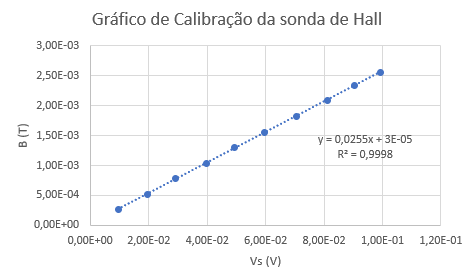
\includegraphics[width=15cm]{./grafico_solenoide.jpeg}
		\caption{Gráfico de calibração da sonda}
	\end{figure}
	
A partir da equação da linearização do gráfico, temos: \\

\begin{equation}
y=2.55*10^{-2}*x + 3*10^-5 
\Leftrightarrow B=2.55*10^-2*Vs + 3*10^-5
\end{equation}
Podemos assim determinar que a constante de proporcionalidade é: \\
\begin{equation}
Cc=2.55*10^-2
\end{equation}
Aplicando o método dos mínimos quadrados temos que a incerteza é: \\

\begin{equation}
\Delta Cc =|Cc|*\sqrt{((1/r^2)-1)/n-2} = |2.55*10^-2|*\sqrt{((1/0.9998^2)-1)/10-2}
\end{equation}

Conclui-se então que: 
\begin{equation}
Cc= 2.55*10^-2 \pm 
\end{equation}


\subsection*{Representação gráfica da variação do campo magnético}
No decorrer da experiência, procedeu-se à variação do campo magnético das bobinas 1 e 2, obtendo assim os seguintes gráficos que apresentam os resultados obtidos:

\begin{figure}[H]
		\centering
		\begin{subfigure}[t]{0.45\textwidth}
			\centering
			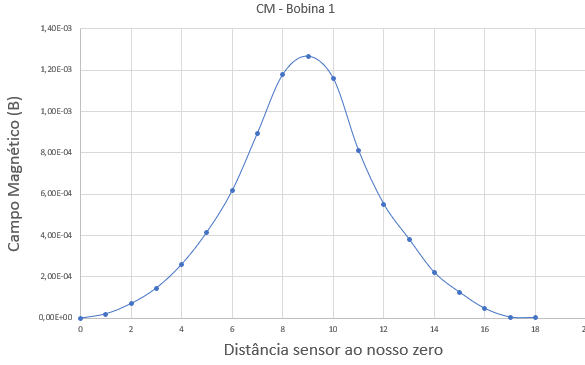
\includegraphics[scale=0.3]{./bobina1.png}
			\caption{}
		\end{subfigure}
		\begin{subfigure}[t]{0.45\textwidth}
			\centering
			{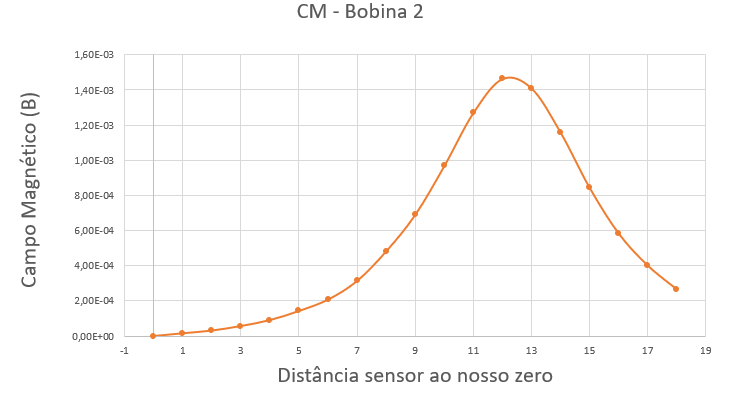
\includegraphics[scale=0.3]{./bobina2.png}}
			\caption{}
			\end{subfigure}	
		\caption{(a) Gráfico de Campo Magnético das Bobinas 1 ; (b) Gráfico de Campo Magnético das Bobinas 2 }
	\end{figure}

\subsection*{Principio de Sobreposição}
\par Considerando o mesmo sentido de corrente, a soma dos gráficos obtidos individualmente para as bobinas 1 e 2, resulta num gráfico semelhante ao obtido quando ambas se encontravam em funcionamento simultâneo (com o mesmo sentido de corrente). \par
A partir desta análise, é possível comprovar que se aplica o princípio de sobreposição, como podemos verificar nos seguintes gráficos:
	
		\begin{figure}[H]
		\centering
		\begin{subfigure}[t]{0.45\textwidth}
			\centering
			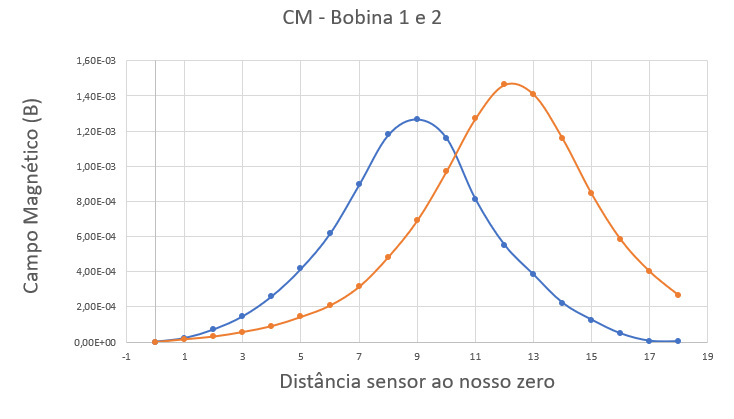
\includegraphics[scale=0.3]{./bobinas1e2.png}
			\caption{}
		\end{subfigure}
		\begin{subfigure}[t]{0.45\textwidth}
			\centering
			{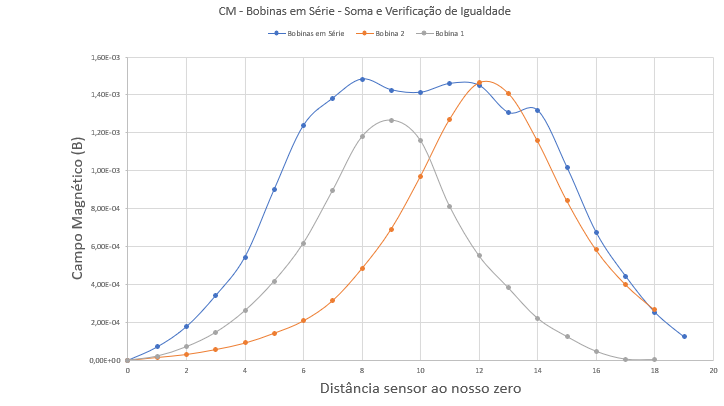
\includegraphics[scale=0.3]{./sobreposição.png}}
			\caption{}
			\end{subfigure}	
		\caption{(a) Gráfico de Campo Magnético das Bobinas 1 e 2 ; (b) Gráfico do Princípio da Sobreposição }
	\end{figure}
		
\subsection*{Estimativa do número de espiras de uma bobina de Helmholtz}

\begin{equation}
B(x)=( \mu /2)*(I*R^2)/(R^2 + (R/2)^2 )^(3/2)
\end{equation}
\begin{equation}
N = (1,40*10^-3/5.96*10^-6) /2 = 123 
\end{equation} , \centering Nº de espiras

\flushleft
\chapter*{Conclusão:}
\par Entre os valores experimentais e os esperados, é possível considerar que ocurreram algumas diferenças, nomeadamente na representação \textbf{Gráfica do Principio de Sobreposição (Figura 5b)}. Podemos constatar que esta representação não é muito fluida, influenciada pelo número de medições que executamos no decorrer da experiencia.
\par Contudo, foi possível verificar que o campo magnético era máximo no seu centro das bobinas e diminuía à medida que a distância ao centro aumentava e demonstrar o princípio de sobreposição.
\par Para o melhorar a experiencia, consideramos relevantes as seguintes alterações futuras:
\begin{itemize}
\item A sonda utilizada para medição do campo não tinha um suporte que a mantivesse fixa num único local, podendo influenciar valores já que constatámos que um simples movimento brusco na mesa influenciava ligeiramente os valores obtidos;
\end{itemize}

\begin{thebibliography}{9}

\bibitem{ibm} 

\textit{Guião Trabalho 2.1.: Bobinas de Helmholtz}. 
Departamento de Física, MCE, Universidade de Aveiro, 2020/21.

\end{thebibliography}
\end{document}